\documentclass{standalone}
\usepackage{tikz}
\usepackage{ctex,siunitx}
\setCJKmainfont{Noto Serif CJK SC}
\usepackage{tkz-euclide}
\usepackage{amsmath}
\usetikzlibrary{patterns, calc,3d}
\usetikzlibrary {decorations.pathmorphing,decorations.pathreplacing,decorations.shapes}
\begin{document}
\small
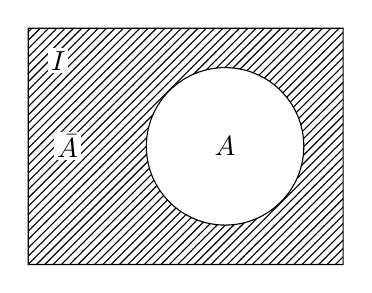
\begin{tikzpicture}[>=latex,scale=1.0,inner sep=1pt]
  \draw[pattern=north east lines,even odd rule](-2.0,1.5)node[below right=10pt,fill=white]{$I$}rectangle(2.0,-1.5)(0.5,0)circle(1.0)node{$A$};
  \node at (-1.5,0)[fill=white]{$\bar{A}$};
\end{tikzpicture}
\end{document}